\chapter{同余}

\begin{introduction}
\item 同余方程
\item 快速乘、快速幂
\item 逆元、线性求区间逆元
\item 中国剩余定理
\item 欧拉降幂
\item 卡米歇尔数
\item Miller\_Rabin
\item Pollard\_Rho
\item 离散对数
\item 原根
\end{introduction}


\section{同余式与同余方程}
\subsection{同余式}
整除性是很好的性质,这在最大公因数、模线性方程和素数分解中均得到了体现。而同余式提供了一种
描述整除性质的简便方式。

\begin{definition}{同余}{label}
	如果$m|(a-b)$,我们就说a与b模m同余并记之为$a\equiv b(mod\ m)$。
	
	特别地,$a\equiv a\%m(mod\ m)$ 。
\end{definition}

数m叫做同余式的模。 具有相同模的同余式在许多方面表现得很像通常的等式。例如:

若$a_1\equiv b_1(mod\ m) \ ,\quad a_2\equiv b_2(mod\ m)$     则$a_1\pm a_2\equiv b_1\pm b_2(mod \ m)$ ,$a_1a_2\equiv b_1b_2(mod \ m)$ 

{\heiti 但 $ac\equiv bc(mod \ m)$ 时,未必有$a\equiv b(mod \ m)$,只有$gcd(c,m)=1$,才可以消去c。}


\subsection{同余方程}
如果同余式含有未知数,我们考虑如何求解。

首先考虑“穷举法” ,要解模m同余式,可让每个变量试取0,1,2...,m-1。例如,解同余式$x^2+2x-1\equiv 0(mod\ 7)$,
就去试$x=0\quad, x=1\quad,...\quad,x=6$,这样可以求出两个解$x\equiv 2(mod\ 7)$和$x\equiv 3(mod\ 7)$ 当然还有其他解,但新的解与2或3是同余的,如9和10。当我们说“求同余式的所有解时”,是指求所有不同余的解,即相互不同余的所有解。

许多同余式是没有解的,如$x^2\equiv 3(mod\ 10)$。

\vbox{}

下面考虑如何求解同余式$ax\equiv c(mod\ m)$。 
\begin{example}
解同余式$18x\equiv8(mod\ 22)$
\end{example}

等价于求$22\ |\ (18x-8)$,即求$18x-22y=8$。       

解这类方程的问题在第一章中研究过。

对于$ax\equiv c(mod\ m)$ ,其有解{\heiti 当且仅当}线性方程$ax-my=c$ 有解。


由前可知,线性方程$ax-my=c$ 有解的充分必要条件是$gcd(a,m)\ |\ c$。

且方程$au+mv=g$ 一定有解 ,设一个解为$(u_0,v_0)$,则有
$$
a\frac{cu_0}{g}+m\frac{cv_0}{g}=c
$$
这说明$x_0= \frac{cu_0}{g}$是同余式$ax\equiv c(mod\ m)$ 的一个解,通解为$x=x_0+k\cdot \frac{m}{g}$。

{\heiti 由于相差m的倍数的任何两个解认为是相同的},所有恰好有$g$个不同的解,这些解通过取$k=0,1,2...,g-1$而得到。将上述过程概述为定理:


\begin{theorem}{线性同余式定理$ax\equiv c(mod\ m)$}{label}
设a,c与m是整数,m>=1,且设$g=gcd(a,m)$。 

(a)  如果$g\nmid c$,则同余式$ax\equiv c(mod\ m)$ 没有解

(b)  如果$g\ |\ c$ ,则同余式$ax\equiv c(mod\ m)$ 恰好有g个不同的解。要求这些解,首先求线性方程$au+mv=g$ 的一个解$(u_0,v_0)$ 
{\heiti (欧几里得回带法,在计算机上递归求得,称为扩展欧几里得算法)} 。则$x_0=(\frac{cu_0}{g}\% \frac{m}{g} + \frac{m}{g}) \% \frac{m}{g}$是$ax\equiv c(mod\ m)$ 的解,不同余解的完全集由
$$
x\equiv x_0+k\cdot \frac{m}{g} \  (mod\ m),\quad k=0,1,2,...,g-1
$$
给出。
\end{theorem}


例如,同余式$943x\equiv 381(mod\ 2576)$ 无解,这是因为$gcd(943,2576) \nmid 381$。

另一方面,同余式$893x\equiv 266(mod\ 2432) $
有19个解,因为$gcd(893,2432)=19,\  19|266$     这个19即为不同余解的个数。

下面解方程$893u-2432v=19$ ,使用欧几里得回带法可以求得解$(u,v)=(79,29)$ ,乘以266/19=14得方程$893x-2432y=266$的解$(x,y)=(1106,406)$ ,
即1106是同余式方程的一个解,这样的互不同余的解共有19个。1106加上2432/19=128的倍数(\%2432)就可得到完全解集。


\begin{remark}
	线性同余式定理最重要的情形是$gcd(a,m)=1$ ,在这种情形下,同余式恰好有一个解。
\end{remark}

\lstinputlisting[language=C++, style=codestyle2]{code03/modequation.cpp}

\vbox{}

对于非线性的同余式,其解“不是很确定”。

我们熟悉的是对于{\heiti 一个d次实系数多项式的实根不超过d个} ,这个结论对于同余式并不成立。

例如$x^2+x\equiv 0(mod\ 6)$ 有4个模6不同的根:0,2,3,5。

但是,{\heiti 当p为素数时,这个结论依然成立:}

\begin{theorem}{模p多项式根定理}{label}
设p为素数,$f(x)=a_0x^d+a_1x^{d-1}+...+a_d$ 是次数为d>=1的整系数多项式,且p不整除$a_0$ ,则同余式$f(x)\equiv 0(mod\ p)$ 最多有d个模p不同余的解。
\end{theorem}

\section{快速乘与快速幂}
快速乘和快速幂作为工具经常在程序设计竞赛中遇见。
\subsection{快速乘}
在$C++$中,变量最多只能表示到$2^{64}-1$这么大,所以如果我们要计算$a*b\%c$,而$a,b$都是接近表示上限的数,这个时候就需要快速乘。
即将$b$按二进制位分解分别加上,时间复杂度为$O(log(b))$。
\lstinputlisting[language=C++, style=codestyle2]{code03/fastmul.cpp}

\subsection{$O(1)$快速乘}
上面的“快速乘”时间是$O(logb)$的,如果是两个63位数相乘(结果long long 存不下),则还有一个巧妙的方法可以简单解决这个问题:

\lstinputlisting[language=C++, style=codestyle2]{code03/o1fastmul.cpp}

首先使用浮点运算来得到$\left\lfloor\frac{a * b}{P}\right\rfloor$的值,显然$a*b-d*p$中的两个乘法都有可能会溢出,但是没关系,因为可以知道其差是一个64bit可容纳的正整数,那么溢出部分的差仅可能为0或者1,最后
特判处理一下即可。	
\begin{note}
	当然,如果编译器支持$int128$的话,可以直接用128位数。
\end{note}

\subsection{快速幂}
现在我们要计算$a^b\%c$,如果乘$b$次,时间复杂度太高,考虑将$b$按照二进制分解,每一位分别计算并乘在一起即可。
时间复杂度为$O(log(b))$。相比于快速乘,只是加法变了乘法。
\lstinputlisting[language=C++, style=codestyle2]{code03/fastexp.cpp}


\section{费马小定理与逆元}
前面我们讨论了关于同余式、同余方程的一些性质,小结一下,互质这个条件很重要。

\begin{itemize}
	\item 对于$ac\equiv bc(mod \ m)$,如果$gcd(c,m)=1$,则可以消去c,得到$a\equiv b(mod \ m)$ 。
	\item 对于同余方程 $ax\equiv c(mod\ m)$,若$gcd(a,m)=1$ ,同余式恰好有一个解。
\end{itemize}

{\heiti 对于式子$ax\equiv c(mod\ m)$,令$c=1$,得$ax\equiv 1(mod\ m)$,若$gcd(a,m)=1$,则方程有唯一解$x_0$,
我们称$x_0$为$a$在模$m$意义下的逆元,常记作$a^{-1}$。}

逆元可以用来说明一些事情,比如如果$ac\equiv bc(mod\ m)$,若$gcd(c,m)=1$,
则存在$c^{-1}$使得$cc^{-1}\equiv 1 (mod\ m)$。所以可以对$ac\equiv bc(mod\ m)$两边同时乘以$c^{-1}$,得到$a\equiv b(mod\ m)$。

如何求解逆元呢?拓展欧几里得即可,因为就是一个同余方程:
\lstinputlisting[language=C++, style=codestyle2]{code03/inverse.cpp}

\vbox{}

若模数是素数,我们还可以用费马小定理求解。

\begin{theorem}{费马小定理}{femat}
	设p是素数,a是任意整数且$p\nmid a$ ,则 $a^{p-1}\equiv 1(mod\ p)$。 
\end{theorem}

在证明费马小定理之前,先来看一个引理。

\begin{lemma}{为证明费马小定理做准备}{forfemat}
	设$p$是素数,a是任何整数且 $p\nmid a$ 则数
	$$
	a,2a,3a,...,(p-1)a\qquad (modp)
	$$
	与数
	$$
	1,2,3,...,(p-1)\qquad (modp)
	$$
	相同,尽管它们的次序不同。
\end{lemma}

\begin{proof}
	数列$a,2a,3a,...,(p-1)a$,包含$p-1$个数,显然没有一个数被$p$整除 ,假设从中取出两个数ja和ka是关于p同余的,即$p|(j-k)a$,
	又p是素数且p不整除a,所以p整除$(j-k)$。但是$|j-k|<p-1 $,所以$j-k=0$,即$j=k$。
	
	这表明,这p-1个数模p不同,由于任何数mod p仅有$p-1$个不同的非零值,证毕。
\end{proof}

\begin{proof}
	费马小定理的证明。
	
	利用该引理\ref{lem:forfemat},即可完成对费马小定理\ref{thm:femat}的证明,将上面引理列到的两组数相乘,可得到
	$$
	a^{p-1} \cdot (p-1)!\equiv (p-1)!   \qquad (modp)
	$$
	由于$(p-1)!$与p互质(显然除了1没有其它公共因子了),可以消去它(本节开头有提到这个性质),则$a^{p-1}\equiv 1(mod\ p)$。
\end{proof}

\vbox{}

有了费马小定理,若模数$m$是质数,则数$a$关于$m$的逆元就是$a^{m-2}$,因为$a* a^{m-2} \equiv 1 \ (mod p)$。
使用快速幂直接计算即可。

\vbox{}

{\heiti 使用费马小定理还可以进行素数测试},后面小节会提到。

\vbox{}

\begin{note}
	如果要求$1,2,3,...,n$所有数的逆元,除了每个单独求之外,实际上还有线性的做法。
	
	设$p=ki+b$ ,那么$ki+b\equiv 0 \ (mod\  p)$。 
	
	两边同乘以$i^{-1},b^{-1}$ 得到$kb^{-1}+i^{-1}\equiv 0 \  (mod\ p)$,$i^{-1}\equiv -kb^{-1}$,于是有:
	
	$$i^{-1}\equiv -\lfloor\frac{p}{i}\rfloor * (p\%i)^{-1} \quad (mod\ p)$$
	
	通常在前面加上$p$,变为正数:
	$$i^{-1}\equiv (p-\lfloor\frac{p}{i}\rfloor) * (p\%i)^{-1} \quad (mod\ p)$$
	
	代码:预处理$1\sim n$的逆元、阶乘和阶乘逆元。时间复杂度为线性。
	\lstinputlisting[language=C++, style=codestyle2]{code03/linearinverse.cpp}
\end{note}

\section{中国剩余定理}

\begin{theorem}{中国剩余定理}{CRT}
	设m与n是整数,$gcd(m,n)=1$,b与c是任意整数,则同余式组
	$x\equiv b(mod\ m)$与$x\equiv c(mod\ n)$恰有一个解$0\leqslant x<mn$。
\end{theorem}

\begin{proof}
	对于第一个同余式$x\equiv b(mod\ m)$,其解由形如$x = my +b$的所有数组成。将其带入第二个方程可得
	$my\equiv c-b (mod\ n)$,已知$gcd(m,n)=1$,由线性同余式定理知其恰有一个解$y_1,\ 0\le y_1<n$,则$x_1=my_1+b$
	给出了原来同余式组的解,这是在$[0,mn)$之间的唯一解。
\end{proof}

\vbox{}

上面只考虑了两个同余式,如果有多个呢?

\begin{custom}{问题}
	求出方程组$x\equiv a_i(mod \ m_i) (0 \leqslant i <n) $ 的解$x$,其中$m_0,m_1,m_2,m_3,...,m_{n-1}$ 两两互质。
\end{custom}

\begin{solution}
	令$M_i=\prod_{j\neq i}m_j$     则有$(M_i,m_i)=1$   
	
	故存在$p_i,q_i$ ,使得$M_i*p_i+m_i*q_i=1$ 
	
	令  $e_i=M_ip_i$,\quad    $p_i$即为$M_i$ 模$m_i$下的逆元。   
	
	则有
$$
e_i\equiv\left\{\begin{matrix}
0(mod\ m_j)\ ,\ j\neq i\\ 
1(mod\ m_j)\ ,\ j=i
\end{matrix}\right.	
$$	
	故$e_0a_0+e_1a_1+e_2a_2+...+e_{n-1}a_{n-1}$是方程的一个解。
	
	由中国剩余定理知,$[0\sim\prod_{i=0}^{n-1}m_i\}$ 中必有一解,将上式模$\prod_{i=0}^{n-1}m_i$即可。 
\end{solution}

时间复杂度  $O(nlogm)$,其中$n$表示有$n$个方程。

\lstinputlisting[language=C++, style=codestyle2]{code03/crt.cpp}

\begin{custom}{问题}
	如果这些方程的{\heiti 模数不互质}呢?(上面互质的方法只是一种巧妙的构造)
\end{custom}

一样可以求解,每一次我们将两个方程合并为一个方程,具体来说,假设目前的前两个方程为$x\equiv a_1 \ (mod\ m_1),\quad  x\equiv a_2 \ (mod\ m_2)$。
将第一个带入第二个可得到$km_1\equiv a_2-a_1 \ (mod\ m_2)$,解这个同余方程,求出$k$的最小正整数解$k_0$,那么$k = \frac{m_2}{gcd}y+ k_0$,带入
$x=km_1+a_1$中可以得到$x=\frac{m_1m_2}{gcd}y+m_1k_0+a_1$,也即将前两个方程合并为了一个:$x\equiv m_1k_0+a_1\ (mod\ \frac{m_1m_2}{gcd})$,
这样迭代下去,最后的那个方程即为所求。

时间复杂度为$nlogm$,其中$n$是方程个数。{\heiti 代码中的$x_0$即为上面的$k_0$。}

\lstinputlisting[language=C++, style=codestyle2]{code03/excrt.cpp}

\section{欧拉公式与欧拉降幂}

\subsection{欧拉公式}

费马小定理很漂亮$a^{p-1}\equiv 1(mod\ p)$,但限制$p$是素数且$p\nmid a$。如果$p$是合数,即使$a,p$互质,结论也不正确了。
那是否有$a^{???}\equiv 1(mod\ m)$成立的指数呢?带规律的那种。
首先,如果a的某个幂模m余1,则a和m必互质(可由线性方程定理证明)。

这再次提醒我们观察与m互素的数的集合:
$$
{a:1\leqslant a\leqslant m,\quad gcd(a,m)=1}
$$
{\heiti 在1$\sim$m之间与m互质的整数个数}是个重要的量,我们赋予这个量一个名称:


\begin{definition}{欧拉函数$\varphi$}{label}
$$
\varphi(m)=\{a:1\leqslant a\leqslant m,\quad gcd(a,m)=1\}
$$
\end{definition}

注意p是素数时,每个整数$1\leqslant a<p$ 都与p互素,所以对于素数p有公式
$$
\varphi(p)=p-1
$$
我们设法模仿费马小定理的证明。例如,假设要求7的幂次模10余1,不取所有1$\sim$9,而是恰好取与10互素的数,它们是
$$
1,3,7,9
$$
如果用7去乘每个数可得
$$
7\cdot 1\equiv 7(mod\ 10)\quad 7\cdot 3\equiv 1(mod\ 10)\quad
7\cdot 7\equiv 9(mod\ 10)\quad 7\cdot9\equiv 3(mod\ 10)
$$
{\heiti 得到的4个数是之前的4个数的重排!}如果将它们乘起来就得到相同的乘积
\begin{align*}
(7\cdot 1)(7\cdot 3)(7\cdot7)(7\cdot9)\equiv 1\cdot3\cdot7\cdot9  \qquad  (mod\ 10)  \\
7^4(1\cdot3\cdot7\cdot9)\equiv 1\cdot3\cdot7\cdot9 \qquad (mod\ 10)
\end{align*}

由于$1\cdot3\cdot7\cdot9$与$10$是互质的,因此可以消去,所以得到$7^4\equiv 1(mod\ 10)$,这个形式和费马小定理很像了!

考虑这里的指数4和费马小定理中的$p-1$的共同点, 都是1$\sim$m中与m互质的数的个数,即欧拉函数$\varphi(m)$。


\begin{theorem}{欧拉公式}{eulerf}
如果$gcd(a,m)=1$ ,则
$$
a^{\varphi(m)}\equiv 1 (mod\ m)
$$
\end{theorem}

\begin{lemma}{为证明欧拉公式做准备}{foreulerf}
如果$gcd(a,m)=1$,则数列
$$
b_1a,\ b_2a,\ b_3a,\ ...\ ,b_{\varphi(m)}a  \qquad  (mod\ m)
$$
与数列
$$
b_1,\ b_2,\ b_3,\ ...\ ,b_{\varphi(m)} \qquad (mod\ m)
$$
相同,尽管它们可能次序不同,$b_i$表示小于$m$且与$m$互质的数。
\end{lemma}

\begin{proof}
引理的证明。
\begin{itemize}
	\item 注意到$b_i$和a均与m是互质的,则$b_ia$也与m互质。{\heiti 又因为所有与m互质的数\%m后依然与m互质} 
	(如果x-km与m不互质,则x与m也不互质了),所以数列$b_1a,b_2a,b_3a,...,b_{\varphi(m)}a  \quad  (mod\ m)$ 同
	余于数列$b_1,b_2,b_3,...,b_{\varphi(m)} \quad (mod\ m)$ 中的某一个数(因为就这$\varphi(m)$个和$m$互质)。又
	每个数列有$\varphi(m)$个数 ,因此,如果能进一步证明第一个数列中的数对于模m互不相同,就可得出两个数列(重排后)
	相同。  
	\item 从第一个数列中任选两个数,假设它们是同余的,那么意味着$m\ |\ a(b_i-b_j)$,由于a,m是互质的,因而
	有$m|b_i-b_j$,又 $b_i ,b_j$在1与m之间,这说明$b_i=b_j$,即第一个数列中的数模m是不同的。引理证毕。
\end{itemize}
\end{proof}


\begin{proof}
欧拉公式的证明。

利用该引理\ref{lem:foreulerf},即可完成对\ref{thm:eulerf}欧拉公式的证明,
由引理知第一个数列中数的乘积等于第二个数列中数的乘积:
$$
(b_1a)\cdot (b_2a)\cdot (b_3a)\cdot \ ...\ \cdot (b_{\varphi(m)}a) \equiv b_1\cdot b_2\cdot b_3 \cdot \cdot \cdot b_{\varphi(m)} \qquad  (mod\ m)
$$
左边提出$\varphi(m)$个a得到  $a^{\varphi(m)}B\equiv B (mod\ m)$,其中$B= b_1 b_2 b_3 \cdot \cdot \cdot b_{\varphi(m)} $。

由于每个$b$与m都是互质的,因此$B$与m也是互质的,因此B可以消去,于是得到
$$
a^{\varphi(m)}\equiv 1 (mod\ m)
$$
证毕。
\end{proof}

关于欧拉函数$\phi$,后面还会遇到。下一节让我们先看一下欧拉公式的一个应用。

\subsection{欧拉降幂}
如何计算$5^{100000000000000}mod\ 12830603$? (实际上会有很多零,比如$10^5$个,这里为了说明问题简写)

如果12830603是素数,则直接使用费马小定理,可以将指数除以p-1,将余数作为幂计算即可。

但12830603=3571*3593,不是素数。

但但,$gcd(5,12830603)=1$,因此由欧拉公式知$5^{\varphi(12830603)}\equiv 1 (mod \ 12830603)$。
计算得到$\varphi(12830603)=12823440$,因此只要把100..000除以12823440的余数作为指数即可。{\heiti 注意这里要求5和12830603互质}。

{\heiti 如果底数和模数不互质呢?有广义欧拉降幂公式},总结如下:

\begin{theorem}{广义欧拉降幂公式}{label}
	\begin{align*}
	a^b\equiv  \left\{\begin{matrix}
	a^{b\% \phi(p)}&  \quad gcd(a,p)=1 \\
	a^b   \quad  & gcd(a,p)\neq 1,b\le \phi(p) \\
	a^{b\% \phi(p)+\phi(p)} &\quad   gcd(a,p)\neq 1,b>\phi(p)
	\end{matrix}\right. \quad {mod \ p}
	\end{align*}
\end{theorem}


\begin{proof}
	第一行和第二行的式子之前已经说明,下面证明$b>\phi(p)$的情况。
	
	设$b = A*\phi(p) + C$,其中$A\ge1,\ 0\le C<\phi(p)$。
	
	那么我们要证明的就是$a^{ A*\phi(p) + C} \equiv  a^{\phi(p)+C}(\ mod\ p)$。
	
	如果我们能证明$a^{A*\phi(p)} \equiv a^{\phi(p)}( mod\ p)$,则上式也就成立。
	
	即证$a^{2*\phi(p)} \equiv a^{\phi(p)}( mod\ p)$,移项即证
	
	$$p\ |\  a^{\phi(p)}(a^{\phi(p)}-1)$$
	
	(这里p不一定是素数)
	
	假设
	$$
	(\frac{p}{(p\ ,\ a^{\phi(p)})}\ ,\ a)= 1
	$$
	
	那么根据欧拉定理,
	$$
	a^{\phi(p)} = a^{k*\phi(\frac{p}{ {(p,a^{\phi(p)})}})}\equiv {[a^{\phi(\frac{p}{ {(p,a^{\phi(p)})}})}]}^k \equiv 1 \ ,\quad mod\ (\frac{p}{(p,a^{\phi(p)})})
	$$
	其中$k\ge 1$,移项可得$\frac{p}{(p,a^{\phi(p)})}\ |\ (a^{\phi(p) }- 1)$。
	两边同时乘${(p,a^{\phi(p)})}$可得$p\ |\  {(p,a^{\phi(p)})}*(a^{\phi(p)}-1)$,于是也就证明了$p\ |\  a^{\phi(p)}(a^{\phi(p)}-1)$。证毕。
	
	但上面的假设还没有证明,实际上这个假设是一定成立的,下面证明。
	
	对$a$和$p$进行质因数分解,
	$$
		a = p^{a_1}_1*p^{a_2}_2*....*p^{a_{t_1}}_{t_1} * q^{b_1}_1* q^{b_2}_2*...* q^{b_{t_2}}_{t_2}
	$$
	
	$$
		p = p^{c_1}_1*p^{c_2}_2*....*p^{c_{t_1}}_{t_1} *  r^{d_1}_1* r^{d_2}_2*...* r^{d_{t_3}}_{t_3}
	$$
	则$(a,p) = p^{min(a_1,c_1)}_1*p^{min(a_2,c_2)}_2*....*p^{{min(a_{t_1},c_{t_1})}}_{t_1}$,
	
	$(a^{\phi(p)},p) =  p^{min(a_1*\phi(p),c_1)}_1*p^{min(a_2*\phi(p),c_2)}_2*....*p^{{min(a_{t_1}*\phi(p),c_{t_1})}}_{t_1}$。
	
	我们分析一下$a_i*\phi(p)$,$a_i*\phi(p)\ge a_i*p_i^{c_i-1}*(p_i-1) \ge p_i^{c_i-1}*(p_i-1) \ge p_i^{c_i-1}\ge c_i$。(其中$p_i$是$p$的因子)。
	
	于是有$(a^{\phi(p)},p) =  p^{min(a_1*\phi(p),c_1)}_1*p^{min(a_2*\phi(p),c_2)}_2*....*p^{{min(a_{t_1}*\phi(p),c_{t_1})}}_{t_1} = p^{c_1}_1*p^{c_2}_2*....*p^{c_{t_1}}_{t_1}$。
	
	于是
	$$
		(\frac{p}{(p\ ,\ a^{\phi(p)})}\ ,\ a)= 1
	$$
	证毕。
\end{proof}

实际上,广义欧拉降幂公式说明的是$a^b\%c$循环节的问题,

这里\href{https://math.stackexchange.com/questions/653682}{https://math.stackexchange.com/questions/653682}
有相关的讨论,$\phi(c)$不一定是最小的循环节长度。

\begin{example}
2019南京网络赛B.superlog,题目经简化后即求$a^{a^{...}} \% m$的值,其中$...$共有$b$个$a$,数据范围是$a,b,m\ \le 10^6$。
\end{example}

由于$m$的范围已知,发现只有很少个形如$a^{a^{...}}$的式子的真值会比$m$小,提前预处理一下即可,这也是比较常见的做法,因为指数套指数增长的非常快。

代码如下,时间复杂度为$O(T*log(m)*\sqrt{m})$。

\lstinputlisting[language=C++, style=codestyle2]{code03/superlog.cpp}


\subsection{威尔逊定理}
在欧拉公式的证明中,我们记$B=b_1b_2b_3...b_{\phi(m)}$,即$B$为小于$m$且与$m$互质的数的乘积。那么我们能给出一个结论,
$B\equiv 1(mod\ m)$或$B\equiv m-1(mod\ m)$。那$m$的模式是怎样的?(即何时为$1$,何时为$m-1$)

\begin{theorem}{威尔逊定理}{wilson}
	将$m$质因数分解,若其形如$2^2,p^k, 2*p^k$中的一种,则$B\equiv m-1(mod\ m)$,否则$B\equiv 1(mod\ m)$,其中$p$为奇素数。
	
	特殊地,若$m$为素数,则$B=(m-1)!$,有$(m-1)! \equiv m-1 \ (mod\ m)$,反过来也成立。
\end{theorem}

威尔逊定理给出了判定一个{\heiti 自然数是否为素数}的充分必要条件,但是由于阶乘是呈爆炸增长的,其结论对于实际操作意义不大。
实际(比赛)中,更常用的是一个叫$Miller\_Rabin$的测试,下面就来看一下如何做素性测试。

\section{素性测试}
素数是整数中优美的一部分,怎么判别一个数是不是素数呢?费马小定理告诉我们$a^p\equiv a \  (\ mod \ p)$,首先,不满足上式的数,一定不是素数。
但就算你尝试了许多$a$之后发现都满足上式,也不能断言$p$就是素数!

确实,对于大部分小的合数$n$,你会发现选取的大部分$a(a<n)$,都不满足费马小定理。
但是!还是有一些合数,比如$561=3*11*17$ ,对所有的$0\leq a < 561$ ,发现都满足费马小定理!

下面证明一下,要证明$a^{561}\equiv a\  (mod \ 561)$,只要证明
\begin{align*}
a^{561}\equiv a\  (mod  \ 3) \ ,\quad a^{561}\equiv a\  (mod  \ 11) \  ,\quad  a^{561}\equiv a\  (mod  \ 17)
\end{align*}
为什么呢?因为若第一个式子成立,则$3 \ |\  a^{561}-a$  ,同理11,17也整除,由于3,11,17互质,则561也整除。
下面就来证明,对于第一个式子,若3能整除a,则显然成立;否则,由于$a^2\equiv 1\ (mod \ 3)$  ,则$a^{561}=a^{2*280+1}=(a^2)^{280}*a\equiv 1*a \equiv  a  \ (mod \ 3)$,
后面两个式子同理。

$561$很特殊!类似这样的数,称为卡米歇尔数。\href{http://oeis.org/A002997/b002997.txt}{http://oeis.org/A002997/b002997.txt}

\subsection{卡米歇尔数}

\begin{definition}{卡米歇尔数}{label}
	卡米歇尔数是这样的合数$n$,即对每个整数$1\le a < n$,都有
	$$
		a^n \equiv a \ (mod \ n)
	$$
\end{definition}

关于卡米歇尔数,存在一些猜想:

{\heiti
\begin{enumerate}
	\item 卡米歇尔数都是奇数;
	\item 卡米歇尔数是不同素数的乘积。
\end{enumerate}
}

\begin{proof}
	对1的证明。
	
	由于$a^n\equiv a \ (mod \ n)$,令$a=n-1$,则可得$(-1)^n\equiv -1 \ (mod \ n)$  则$n$是奇数。
\end{proof}

\begin{proof}
	对2的证明。
	
	假设卡米歇尔数的任意一个素因子(次幂)为$p^{(e+1)}$ ,下面我们努力证明$e=0$。
	
	将$p^e$带入$a^n\equiv a \ (mod \ n)$,得到$p^{en}\equiv p^e \ (mod \ n)$,所以$n \ | \ p^{en}-p^e$,又$p^{e+1} \ | \ n$,所以$p^{e+1} \ | \ p^{en}-p^e$,
	从而$e=0$。证毕。
\end{proof}


\begin{theorem}{卡米歇尔数的考塞特判别法}{kamixieer}
	设n是合数,则n是卡米歇尔数当且仅当它是奇数,且整除n的每个素数$p$满足下述两个条件:(充分必要)
	\begin{itemize}
		\item $p^2 $不整除n
		\item $p-1$整除$n-1$ (实际上整除更小的数$\frac{n}{p}-1$)
	\end{itemize}
\end{theorem}

利用考塞特判别法,我们可以在$O(\sqrt{n})$的时间内处理单个数的判别以及$O(T*n)$求区间carmichael数,其中$T$表示大常数。

下面的代码求出$\le 10^7$的所有carmichael数。
\lstinputlisting[language=C++, style=codestyle2]{code03/carmichael.cpp}

1994年,W.R.Alford等人证明了卡米歇尔数有无穷多个。

卡米歇尔数的存在,使得我们需要一个更好的检验合数的办法。

\subsection{Miller\_Rabin测试}
合数的miller\_rabin测试是基于以下事实的:

\begin{theorem}{素数的一个性质}{label}
设$p$是奇素数,记$p-1=2^kq$ ,$q$是奇数,{\heiti 设$a$是不被$p$整除的任何数},则下述两个条件之一一定成立:(但满足条件之一的数不一定是素数,卡米歇尔数)
\begin{itemize}
	\item $a^q$模$p$余1
	\item 数$a^q,a^{2q},a^{2^2q},...,a^{2^{k-1}q}$之一模$p$余$-1$
\end{itemize}
\end{theorem}

\begin{proof}
	费马小定理告诉我们$a^{p-1}\equiv 1\ (mod \ p)$。这意味着对于数表$a^q,a^{2q},a^{2^2q},...,a^{2^{k-1}q},a^{2^kq}$ ,最后一个数模$p$余1,且表中的每个数是前一个数的平方。因此下述两种可能之一必成立:
\begin{itemize}
	\item 表中的第一个数模$p$余1
	\item 表中的一些数模$p$不余1,但是,当平方时它就模$p$余1,所以该数是$-1(mod \ p)$,即表包含$-1(mod \ p)$
\end{itemize}
	证毕。
\end{proof}

\begin{theorem}{miller\_rabin测试}{label}
	设$n$是奇素数,记$n-1=2^kq$,$q$是奇数,对不被$n$整除的某个$a$,如果下述{\heiti 两个条件都成立},则$n$一定是合数:(但有不成立的也不一定是素数,于是可以做多次...)
	\begin{itemize}
		\item $a^q \not\equiv 1 \ (mod \ n)$
		\item 对所有的$i=0,1,2,...,k-1 ,\quad a^{2^iq}\not\equiv -1\ (mod \ n)$
	\end{itemize}
\end{theorem}
和费马小定理测试相比,miller\_rabin测试不存在“卡米歇尔型数”,因为可以保证,如果$n$是奇合数,则1$\sim$n-1之间至少有约75\%的
数可作为miller\_rabin的证据。即这些数作为$a$时,可以说明其合数性。

{\heiti 换句话说,每个合数都有许多证据来说明它的合数性。}

例如随机选取100个$a$的值,若实验发现其中均没有$n$的miller\_rabin证据(两个条件一直都有不成立的),则$n$是合数的概率小于$0.25^{100}$。


时间复杂度:$O(T*logn*logn)$ ,其中$T$为测试次数,(如果$n>10^9$,需要使用快速乘,认为是两个$log$)。
\lstinputlisting[language=C++, style=codestyle2]{code03/miller.cpp}

\section{Pollard\_Rho质因数分解}

Pollard\_Rho算法是一种用于质因数分解的算法,对于一个待分解的数$N$,假设$N$的最小的质因数为$p(p\neq N)$,那么Pollard\_Rho算法
能够在$O(\sqrt{p}*\alpha(N))$的期望时间复杂度内将$N$分解为两个不是1的数的乘积,其中$\alpha(N)$是求解两个数的gcd的时间复杂度,而且
其不需要额外的空间!下面我们就来看一下它是怎么工作的。

我们之前质因数分解的方法就是去拿$1\sim \sqrt{N}$的所有数去试除,那如果$N$是$10^{18}$,就顶不住了。其实,可以随机去做这件事,如果运气好的话,
就可以将一个数分解为两个数相乘($\frac{1}{\sqrt{N}}$的概率)。有没有更好的方法,使得猜中其因数的概率增大呢?

我们先来考虑这样一个问题:在$[1,1000]$里随机选择一个数,是$23$的概率是多少?显然是$\frac{1}{1000}$,那如果我们选择两个数$i,j$,$|i-j|=23$的概率是多少?
答案大概是$\frac{1}{500}$。这给了我们一点启发,这种“多点采样”的方法,是否能提高选中目标的概率?著名的生日悖论就是这种思想!

假如说班上有$k$个人,如果找到一个人的生日是2月3日,这个概率比较低。但是如果单纯想找到两个生日相同的人,这个概率就会很高!
由高中的数学知识知道,$k$个人生日互不相同,其概率为:$p=\frac{365}{365}*\frac{364}{365}*\frac{363}{365}*...*\frac{365-k+1}{365}$,
故生日有重复的现象的概率是$P(k) = 1 - \Pi_{i=1}^k\frac{365-i+1}{365}$。当$P(k)\ge\frac{1}{2}$时,解得$k$大概只需要23。
当$k$取到$60$时,$P(k)\approx 0.9999$。这可能和我们的直觉不符,因此被称为悖论。

现在回到因数分解的问题上,由于一定有$gcd(k,n)\ |\ n$,如果我们通过一些组合选取适当的$k$,有$gcd(k,n)>1$,就找到了一个$n$的因数!
这样的$k$的数量还是蛮多的,假设$n$有若干个质因子,则每个质因子的倍数都是可行的(简单一想,至少得有$O(\sqrt{n})$个吧)。
于是,我们可以选取一组数$x_1,x_2,...,x_n$,若有$gcd(|x_i-x_j|,N)>1$,则$gcd(|x_i-x_j|,N)$是$N$的一个因子。
有前人在论文中指出,要使概率接近1,需要选取的数的个数大约是$O(N^{\frac{1}{4}})$。但是如果要$O(n^2)$枚举两两计算,还不如直接$\sqrt{N}$暴力。

我们不妨考虑构造一个伪随机数序列,然后取相邻的两项做差来求$gcd$,这样时间复杂度就降了下来。{\heiti 为了生成一串优秀的随机数},$Pollard$设计了这样一个函数:
$f(x) = (x^2+c)  \ mod\ N$,其中$c$是一个随机的常数。之所以叫伪随机数,是因为这个序列里可能会含有循环,比如取$c=7, N=20, x_1=1$,序列为$1,8,11,8,11,8,...$。
循环节的产生很自然,在模$N$的意义下,函数的值域为$0,1,2...,N-1$,只要有一次序列的值之前出现过,那么序列就会开始循环。如果画出这个序列,并让循环的地方指向之前,其轨迹
很像一个希腊字母$\rho$。(算法名字的由来)

为了方便地判断环的存在,可以用{\heiti 快慢指针}。

考虑有一个单链表,其中可能有一个环,也就是某个节点的next指向的是链表中在它之前的节点,这样在链表的尾部会形成环,如图\ref{fig:Fast-and-slow-pointer}。
现在有两个指针都指向开始节点$A$,然后向右移动,一个一次移动一个节点,另外一个一次移动两个节点,假设相遇在$P$点,那么可以证明一定有$P->B$的长度等于$A->B$。
对于上面的伪随机数序列,有$A->P$(不包含$P$)为一个完整的循环节。于是我们可以设置两个变量,一个变量每次向后迭代一次,而另一个每次向后迭代计算两次,在这两个
变量相等之前,取它们的差用于求$GCD$。

\begin{figure}[htbp]
	\centering
	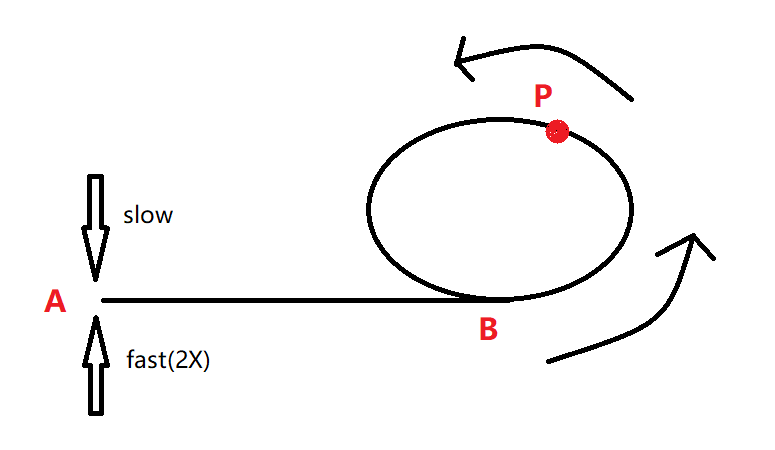
\includegraphics[width=0.7\textwidth]{Fast-and-slow-pointer.png}
	\caption{Fast-and-slow-pointer \label{fig:Fast-and-slow-pointer}}
\end{figure}

代码如下:
\lstinputlisting[language=C++, style=codestyle2]{code03/pollard-rho.cpp}

由于求$GCD$大概会有一个常数,考虑进一步优化。显然如果我们能求得$gcd(ab,N)>1$,那么也是找到了一个因子,只要$a,b$中某一个有$N$的因子即可。
所以我们可以先不急着做$GCD$,而是做一系列的$|t-s|$的连乘,到一定次数再做$GCD$。为了不溢出,我们使连乘的结果$mod\ N$,由欧几里得算法知答案不变。

\lstinputlisting[language=C++, style=codestyle2]{code03/pollard-rho-with-multi.cpp}

pollard-rho算法往往会和miller-rabin同时使用,比如章节题目\ref{prob:pollard}。
其要判断一个数是否是素数,若不是则输出其最大质因子。

代码如下,可作为模板,时间复杂度$O(T*\alpha*(N^{1\over 4}+log^2(N)))$。其中$T$表示数据组数,$\alpha$表示一个不小的常数。

\lstinputlisting[language=C++, style=codestyle2]{code03/luogu-p4718.cpp}

\section{离散对数}

现在我们来思考这样一个问题:

\begin{custom}{问题}
	给定$a,b,m$,求$a^x\equiv b \ (mod \ m)$的解$x$。
\end{custom}

\begin{solution}
	
	我们设$x=A\left \lceil \sqrt{m} \right \rceil -B$,其中$0\le B< \left \lceil \sqrt{m} \right \rceil$, $0< A\le \left \lceil \sqrt{m} \right \rceil+1$,这样化简后的方程是
	$$
	a^{A\left \lceil \sqrt{m} \right \rceil}\equiv b\cdot a^B \quad (mod \ m)
	$$
	由于$A$和$B$值域都是$O(\sqrt{m})$级别的,所以可以先计算右边部分的值,存入$Hash$表,然后从小到大枚举$A$计算左边的值,在$Hash$表中查找。
	(当然,可以这样做的原因是一定存在$a$的逆元)即只要$gcd(a,m)=1$,上面的方法就是有效的。所以当$m$是质数时,用这种方法(Baby Step Giant Step, bsgs)即可。
	
	{\heiti 当$m$不是质数时},我们要求解的是$a^x+km=b$,设$g=gcd(a,m)$,如果$g$不整除$b$,则无解,否则方程两边同除以$g$,得到$\frac{a}{g}a^{x-1}+k\frac{m}{g}=\frac{b}{g}$。
	这样便消去了m的一个因子,得到方程
	$$
	\frac{a}{g}a^{x-1}\equiv \frac{b}{g}\quad (mod \   \frac{m}{g})
	$$
	令${m}'=\frac{m}{g} ,\ b'=\frac{b}{g}(\frac{a}{g})^{-1}$, 得到
	$$
	a^{x'}\equiv b' \quad (mod \ m')
	$$
	于是可以递归,得到的解加1即$x=x'+1$为原方程的解。
	
	{\heiti 但是,进行一次这样的操作,新的方程不一定可以用bsgs求解,所以会进行多次。}
	
	如果中途出现$b'=1$则$x'=0$。
\end{solution}

时间复杂度  $O(\sqrt{m}log\sqrt{m})$,手写二分比unordered\_map会快一点。

\lstinputlisting[language=C++, style=codestyle2]{code03/bsgs.cpp}

注意到代码中有一个技巧,不用把每一步的逆元实际求出来,放到式子左边乘起来就行。
查表时,把初值设置为这个数$*a^{\left \lceil \sqrt{m} \right \rceil}$即可。


\section{原根}
\subsection{幂模$p$与原根}

如果$a$和$p$互素,费马小定理告诉我们,$a^{p-1} \equiv 1\ (mod\ p)$,那么这个指数$p-1$是唯一的使得结果为1的吗?
我们选择一些$a$和$p$来看一下,对于$a=3,p=7$,指数只有为6时才取到1,如表\ref{tab:root}。


\begin{table}[!htbp]
	\centering
	\caption{$a=3,\ p=7$ \label{tab:root}}
	\begin{tabular}{ccc}
		\midrule
		 $3^1\equiv 3(mod\ 7)$  & $3^2\equiv 2(mod\ 7)$ & $3^3\equiv 6(mod\ 7)$ \\
		 $3^4\equiv 4(mod\ 7)$    & $3^5\equiv 5(mod\ 7)$ & $3^6\equiv 1(mod\ 7)$ \\
		 \bottomrule
	\end{tabular}%
\end{table}%

再列多一点,如表\ref{tab:root2},从表中可以看出,似乎有这样的性质:
\begin{itemize}
	\item 对于任何底数,最小指数$e$整除$p-1$;
	\item 总有一些底数,指数需要到$p-1$。
\end{itemize}

\begin{table}[!htbp]
	\centering
	\caption{不同底数对应的最小指数 \label{tab:root2}}
	\begin{tabular}{ccc}
		\toprule
		$p=5$  & $p=7$ & $p=11$ \\
		\midrule
		$1^1\equiv 1(mod\ 5)$  & $1^1\equiv 1(mod\ 7)$ & $1^1\equiv 1(mod\ 11)$ \\
		$2^4\equiv 1(mod\ 5)$    & $2^3\equiv 1(mod\ 7)$ & $2^{10}\equiv 1(mod\ 11)$ \\
		$3^4\equiv 1(mod\ 5)$  & $3^6\equiv 1(mod\ 7)$ & $3^5\equiv 1(mod\ 11)$ \\
		$4^2\equiv 1(mod\ 5)$    & $4^3\equiv 1(mod\ 7)$ & $4^5\equiv 1(mod\ 11)$ \\
	                             & $5^6\equiv 1(mod\ 7)$ & $5^5\equiv 1(mod\ 11)$ \\
		    					& $6^2\equiv 1(mod\ 7)$ & $6^{10}\equiv 1(mod\ 11)$ \\
		  											& & $7^{10}\equiv 1(mod\ 11)$ \\
		   			  								& & $8^{10}\equiv 1(mod\ 11)$ \\
		   			  								& & $9^{5}\equiv 1(mod\ 11)$ \\
		   			  								& & $10^{2}\equiv 1(mod\ 11)$ \\
		\bottomrule
	\end{tabular}%
\end{table}%


为了方便,我们定义$a$模$p$的阶指$e_p(a)=[min\ e\ s.t.\ a^e\equiv 1(mod \ p)]$,其中$a$和$p$互质。另外,规定$e_p(a)\ge 1$,显然$e_p(a)\le p-1$。

\begin{theorem}{次数整除性质}{label}
	设a是不被素数$p$整除的整数,假设$a^n \equiv 1 \ (mod \ p)$,则次数$e_p(a)$整除$n$,特别地$e_p(a)$总整除$p-1$。
\end{theorem}

\begin{proof}
	次数$e_p(a)$的定义告诉我们
	$$
	a^{e_p(a)}\equiv 1 \ (mod \ p)
	$$
	假设$a^n\equiv 1(\ mod \ p)$,
	设$G=gcd(e_p(a),n)$,
	并设$(u,v)$是方程$e_p(a)u-nv=G$的正整数解(可知一定有解)。现在有两种不同的方法计算$a^{e_p(a)u}$:
	\begin{align*}
		a^{e_p(a)u}=(a^{e_p(a)})^u\equiv 1 \ (mod \ p)  \\
		a^{e_p(a)u}=a^{nv+G}\equiv a^G \ (mod \ p)  \\
	\end{align*}

	这表明$a^G\equiv 1 (\ mod \ p)$ ,所以必有$e_p(a)\le G$。
	
	另一方面$G \ | \ e_p(a)$,所以$G=e_p(a)\ ,\ e_p(a)\ | \ n$,证毕。
\end{proof}

{\heiti 现在我们的一个猜想得到了证明,来看另外一个:$e_p(a)=p-1$的底数$a$有什么规律。}

如果a是这样的数,则幂
$$
a^1,\ a^2,\ a^3,\ ...\ ,\ a^{p-2},\ a^{p-1}\quad (\ mod \ p)
$$
{\heiti 必须都是模$p$不同的。}[如果幂不是全不相同,则对某指数$1\le i <j\le p-1$有$a^i\equiv a^j \ (mod \ p)$,由于a,p互质,则有$1\equiv a^{j-i} \ (mod \ p)$,由于$j-i<p-1$,则矛盾]。

{\heiti 这$p-1$个不同的数取遍了$[1,p-1]$。}

{\heiti 这样的数很重要,为了方便,我们称这样的数$g$为模数$p$的原根,即$e_p(g)=p-1$。}

回顾前面的那张表\ref{tab:root2},5的原根是2,3\quad ;\quad 7的原根是3,5\quad ;\quad 11的原根是2,6,7,8。
可见原根可以不止一个,那到底有多少个?所有素数都有原根吗?

\begin{theorem}{原根定理}{label}
每个素数$p$都有原根。更精确地,有恰好$\varphi(p-1)$个原根。
\end{theorem}

神奇!尽管原根定理没有指出求$p$的原根的具体方法,但一旦能求得一个原根,就可以容易得求出其他原根(后面介绍)。求原根的常用方法是从小到大枚举正整数a=2,3,5,6......。{\heiti 因为原根的分布比较广}。(思考为什么没有4)。
为啥没4?因为$4^{\frac{(p-1)}{2}}\equiv 2^{p-1}\equiv 1 \ (mod \ p)$,即4一定不是原根。(可见2的高次幂都不是)

\begin{proof}
	原根定理的证明。
	
	对$1\sim p-1$之间的每个数$a$,$e_p(a) \ | \ (p-1)$ ,所以,对整数$p-1$的每个因子$d$,我们可能会问,有多少个$e_p(a)$等于$d$,由于要用,我们记这个数为$\psi (d),\ 1\le a <p$。 
	$\psi(p-1)$即为模数$p$的原根个数。
	
	设$n$是整除$p-1$的任何数,比如说$p-1=nk$,则可将多项式$X^{p-1}-1$分解成$X^{nk}-1=(X^n)^k-1=(X^n-1)((X^n)^{k-1}+(X^n)^{k-2}+...+(X^n)^2+X^n+1)$
	
	我们数一下这些多项式模$p$有多少个根。
	
	首先,$X^{p-1}-1\equiv 0 \ (mod \ p)$恰好有$p-1$个解,即$[1,p-1]$这些。
	
	另一方面,$(X^n-1)\equiv 0 \ (mod \ p)$至多有$n$个解,且
	$$
	(X^n)^{k-1}+(X^n)^{k-2}+...+(X^n)^2+X^n+1 \equiv 0 \ (mod \ p)
	$$
	至多有$nk-n$个解。
	
	因此我们得到:
	\begin{figure}[htbp]
		\centering
		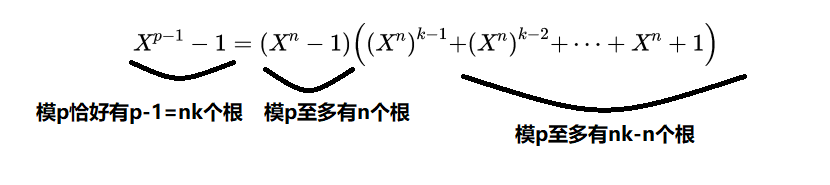
\includegraphics[width=0.7\textwidth]{prime-root.png}
		\caption{根的情况 \label{fig:prime-root}}
	\end{figure}

	上式要成立,$X^n-1$模$p$恰有$n$个根。这就证明了下述重要事实:
	
	{\heiti 如果$n \ | \ p-1$,则同余式$X^n-1\equiv 0 \ (mod \ p)$恰好有$n$个根满足$0\le X<p$。}
	
	现在再用另一种计数方法计数这个同余式的解的个数。如果$X=a$是一个解,则$a^n\equiv 1\ (mod \ p)$,因此$e_p(a)\ | \ n$,即$e_p(a)$对应$n$的一个因子$d$。
	从这个角度,$X^n-1\equiv 0 \ (mod \ p)$解($0\le X<p$)的个数等于:
	$$
		\sum_{d|n}\psi(d)=\psi(d_1)+\psi(d_2)+...+\psi(d_r)
	$$
	
	综合上面两个角度,我们得到一个结论:
	\begin{center}
	{\heiti 若$n$整除$p-1$,则$\sum_{d|n}\psi(d)=n$}
	\end{center}

	
	这个公式和欧拉函数的形式一样!首先,$\varphi(1)=1$,而$\psi(1)=1$,下面证明当$n=q$为素数时,$\psi(n)=\varphi(n)$。
	q的因数是1和q,所以$\psi(q)+\psi(1)=q=\varphi(q)+\varphi(1)$,由于$\psi(1)=\varphi(1)$,则$\psi(q)=\varphi(q)$。$n=q^2$和$n=q_1q_2$也可以类似证明。
	更正式地,可以给出归纳证明,这里不展示了。
	
	证毕。
\end{proof}

{\heiti 综上,我们已证明对整除$p-1$的每个整数$n$,恰好有$\varphi(n)$个底数$a$使得$e_p(a)=n$,取$n=p-1$,则$\varphi(p-1)$为原根个数。显然,每个素数至少有一个原根。}

\vbox{}

{\heiti 求原根,时间复杂度: 对于单个$p$,$O(\sqrt{p} + T*logn*logn)$   ;对于区间问题,可以做到$O(nlogn + \frac{n}{logn}*T*logn*logn)$,其中$T$表示平均意义下每个素数最小原根。
除以$logn$是因为素数的分布。}
\lstinputlisting[language=C++, style=codestyle2]{code03/primitive-root.cpp}

\subsection{原根与指标}
我们大概知道原根是啥了,那指标是什么呢?对于模数13,2是它的原根,那么$2^x\ mod \ 13$会取遍$[1,12]$里所有的数,$x\in [1,12]$。
{\heiti 而指标函数$I$就是从余数到指数的双射函数。}比如$2^4\equiv 3\ (mod\ 13)$,则$I(3) = 4$。



\begin{theorem}{指标法则}{label}
	指标满足下述法则:
		\begin{itemize}
			\item $I(ab)\equiv I(a)+I(b) \quad (mod \ p-1)$ \quad  乘积法则
			\item $I(a^k)\equiv k*I(a)  \quad (mod \ p-1)$ \quad  幂法则
		\end{itemize}
\end{theorem}

\begin{note}
	模数是$p-1$。
\end{note}

\vbox{}

\begin{proof}
	 $g^{I(ab)}\equiv ab\equiv g^{I(a)}g^{I(b)}\equiv g^{I(a)+I(b)}\quad (mod \ p)$
	
	这意味着$g^{I(ab)-I(a)-I(b)}\equiv 1\ (mod \ p)$,又$g$是原根,则$I(ab)-I(a)-I(b)$是$p-1$的倍数。
	
	所以乘积法则得证。幂法则同理。
\end{proof}

\vbox{}

利用指标这个工具,可以方便地解一些高次同余方程。

\begin{custom}{问题}
求同余式$3x^{30}\equiv 4\ (mod \ 37)$。
\end{custom}

\begin{solution}
	使用乘积法则和幂法则:
$$
\begin{aligned} I\left(3 x^{30}\right) &=I(4) \\ I(3)+30 I(x) & \equiv I(4)(\bmod 36) \\ 26+30 I(x) &\equiv2(\bmod 36) \\ 30 I(x) & \equiv-24\equiv12(\bmod 36) \end{aligned}
$$
对于最后一个式子,是一个同余方程,由于$gcd(30,36)=6\ |\ 12$,则其有解,且有6个不同余解。
我们求得
$$
I(x)\equiv 4,\ 10,\ 16,\ 22,\ 28,\ 34 \quad (mod \ 36)
$$
再查双射表得到对应的值,有6个解$16,\ 25,\ 9,\ 21,\ 12,\ 28$。
\end{solution}

可以看到指标法的优点在于将{\heiti 幂运算转为乘法,将乘法转为加法}。这一点和对数函数很像:
$$
\begin{aligned} \log (a b) &=\log (a)+\log (b) \\ \log \left(a^{k}\right) &=k \log (a) \end{aligned}
$$

类似这一题的同余式称为剩余问题,下一章我们就来研究一下。这一章就到这。


\vbox{}

\vbox{}

\begin{problemset}
	\item \href{http://poj.org/problem?id=2891}{Strange Way to Express Integers \quad POJ2891 \quad 同余方程组,模数不一定互质}  
	\item \href{https://cn.vjudge.net/problem/Gym-101550E#}{Exponial \quad 欧拉降幂}
	\item \href{http://acm.hdu.edu.cn/showproblem.php?pid=4910}{Problem about GCD \quad 威尔逊定理的应用}
	\item \href{https://vjudge.net/problem/HDU-5391}{Zball in Tina Town \quad 威尔逊定理 \quad 素性测试}
	\item \href{https://www.luogu.org/problem/P4718}{【模板】Pollard-Rho算法 \quad 素性测试 \quad Pollard\_Rho质因数分解 \label{prob:pollard}}
	\item \href{https://www.spoj.com/problems/MOD/}{MOD - Power Modulo Inverted \quad 离散对数}
	\item \href{http://acm.hdu.edu.cn/showproblem.php?pid=6632}{discrete logarithm problem \quad 模数特殊的离散对数问题}
	\item 对任何正整数$k$,求$1^k+2^k+3^k+...+(p-1)^k\ (mod\ p)$的值。 \  ans:0 \href{https://math.stackexchange.com/questions/1049420/for-any-positive-number-k-find-the-value-of-1k-2k-3k-p-1kmod?r=SearchResults#}{solution}
	\item (2017四川省赛K.2017)给你$n$(不超过200w)个数,和一个数$r$,问你有多少种方案,使得你取出某个子集,能够让它们的乘积$mod \ 2017$等于$r$。由于
	方案数众多,最后只需要输出答案的奇偶性即可。\href{https://www.cnblogs.com/autsky-jadek/p/7496328.html}{\quad 原根}
\end{problemset}

